\documentclass[../main.tex]{subfiles}
\usepackage{listings}
\begin{document}


\subsection{Transformación 1}

La primera transformación nos va a hacer un acción sencilla como pasarnos el xml a html. Nos mostrará en html una vista de todos los medicamentos con sus datos.
\lstset{language=XML}
\begin{lstlisting}
<?xml version="1.0" encoding="UTF-8"?>
<xsl:stylesheet version="1.0"
xmlns:xsl="http://www.w3.org/1999/XSL/Transform">
<xsl:template match="/">
  <html>
    <body>
        <h1>Listado de medicamentos:</h1>
        <ul>
            <xsl:for-each select = "dataset/record">
                <li><h2>Registro: <xsl:value-of select = "NUMERO_DE_REGISTRO"/></h2></li>
                <ul>
                    <li><h3>Información del medicamento</h3></li>
                    <table border = "1">
                        <tr bgcolor="#ff6d6d">
                            <th>Nombre</th>
                            <th>Principios activos</th>
                            <th>Laboratorio</th>
                            <th>Prescripcion</th>
                            <th>Vias de administración</th>
                            <th>Forma farmaucetica</th>
                            <th>Dosis</th>
                            <th>Con receta</th>
                            
                        </tr>
                        <tr>
                            <td><xsl:value-of select = "MEDICAMENTO"/></td>
                            <td><xsl:value-of select = "PRINCIPIOS_ACTIVOS"/></td>
                            <td><xsl:value-of select = "LABORATORIO_TITULAR"/></td>
                            <td><xsl:value-of select = "PRESCRIPCION"/></td>
                            <td><xsl:value-of select = "VIAS_DE_ADMINISTRACION"/></td>
                            <td><xsl:value-of select = "FORMA_FARMACEUTICA"/></td>
                            <td><xsl:value-of select = "DOSIS"/></td>
                            <td><xsl:value-of select = "CON_RECETA"/></td>
                        </tr>
                    </table>
                </ul>
            </xsl:for-each>
        </ul>
    </body>
  </html>
</xsl:template>
</xsl:stylesheet>
\end{lstlisting}

\begin{figure}[h]
    \centering
    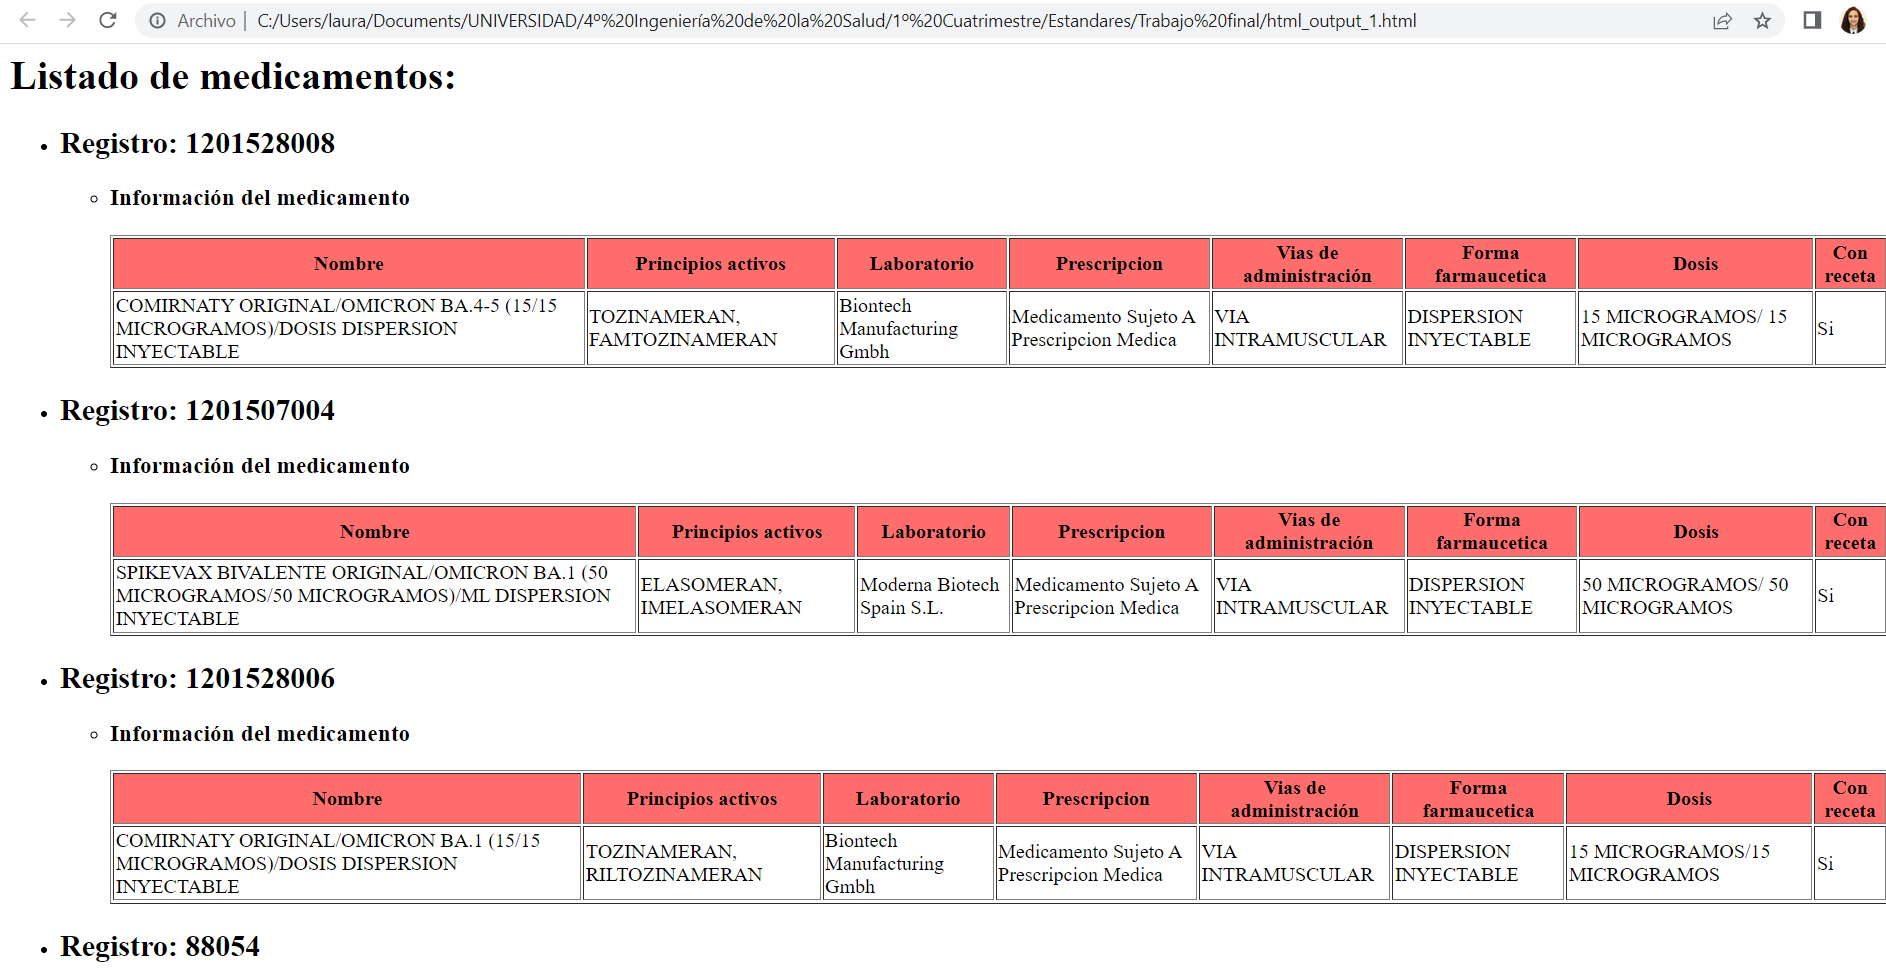
\includegraphics[scale=0.3]{images/html_output1.PNG}
    \caption{Archivo html resultante al aplicar la primera transformación}
    \label{fig:mesh1}
\end{figure}



\subsection{Transformación 2}
La segunda transformación que se ha realizado muestra un listado de todos los medicamentos que tienen una vía de administración oral y cuyo nombre empiece por Aripiprazol.

\begin{lstlisting}
<?xml version="1.0" encoding="UTF-8"?>

<xsl:stylesheet xmlns:xsl="http://www.w3.org/1999/XSL/Transform" version="1.0">
    <xsl:template match="/">
        <html>
            <body>
                <h1> Listado de medicamentos con via de administracion oral y empiezen por aripiprazol</h1>
                <ul>
                    <xsl:for-each select="dataset/record">
                        <xsl:if test="starts-with(MEDICAMENTO,'ARIPIPRAZOL') ">
                            <xsl:if test="contains(VIAS_DE_ADMINISTRACION,'VIA ORAL') ">
                                <li>
                                    <h3> Informacion del medicamento </h3>
                                    <table border="1">
                                        <tr bgcolor="#ff6d6d">
                                            <th> Numero de Registro</th>
                                            <th> Nombre del medicamento</th>
                                            <th> Via de Administración </th>
                                        </tr>
                                        <tr>
                                            <td>
                                                <xsl:value-of select="NUMERO_DE_REGISTRO" />
                                            </td>
                                            <td>
                                                <xsl:value-of select="MEDICAMENTO" />
                                            </td>
                                            <td>
                                                <xsl:value-of select="VIAS_DE_ADMINISTRACION" />
                                            </td>
                                        </tr>

                                    </table>
                                </li>
                            </xsl:if>
                        </xsl:if>
                    </xsl:for-each>
                </ul>
            </body>
        </html>
    </xsl:template>
</xsl:stylesheet>
\end{lstlisting}
El archivo html resultante al aplicar esta transformación es el siguiente:

\begin{figure}[h]
    \centering
    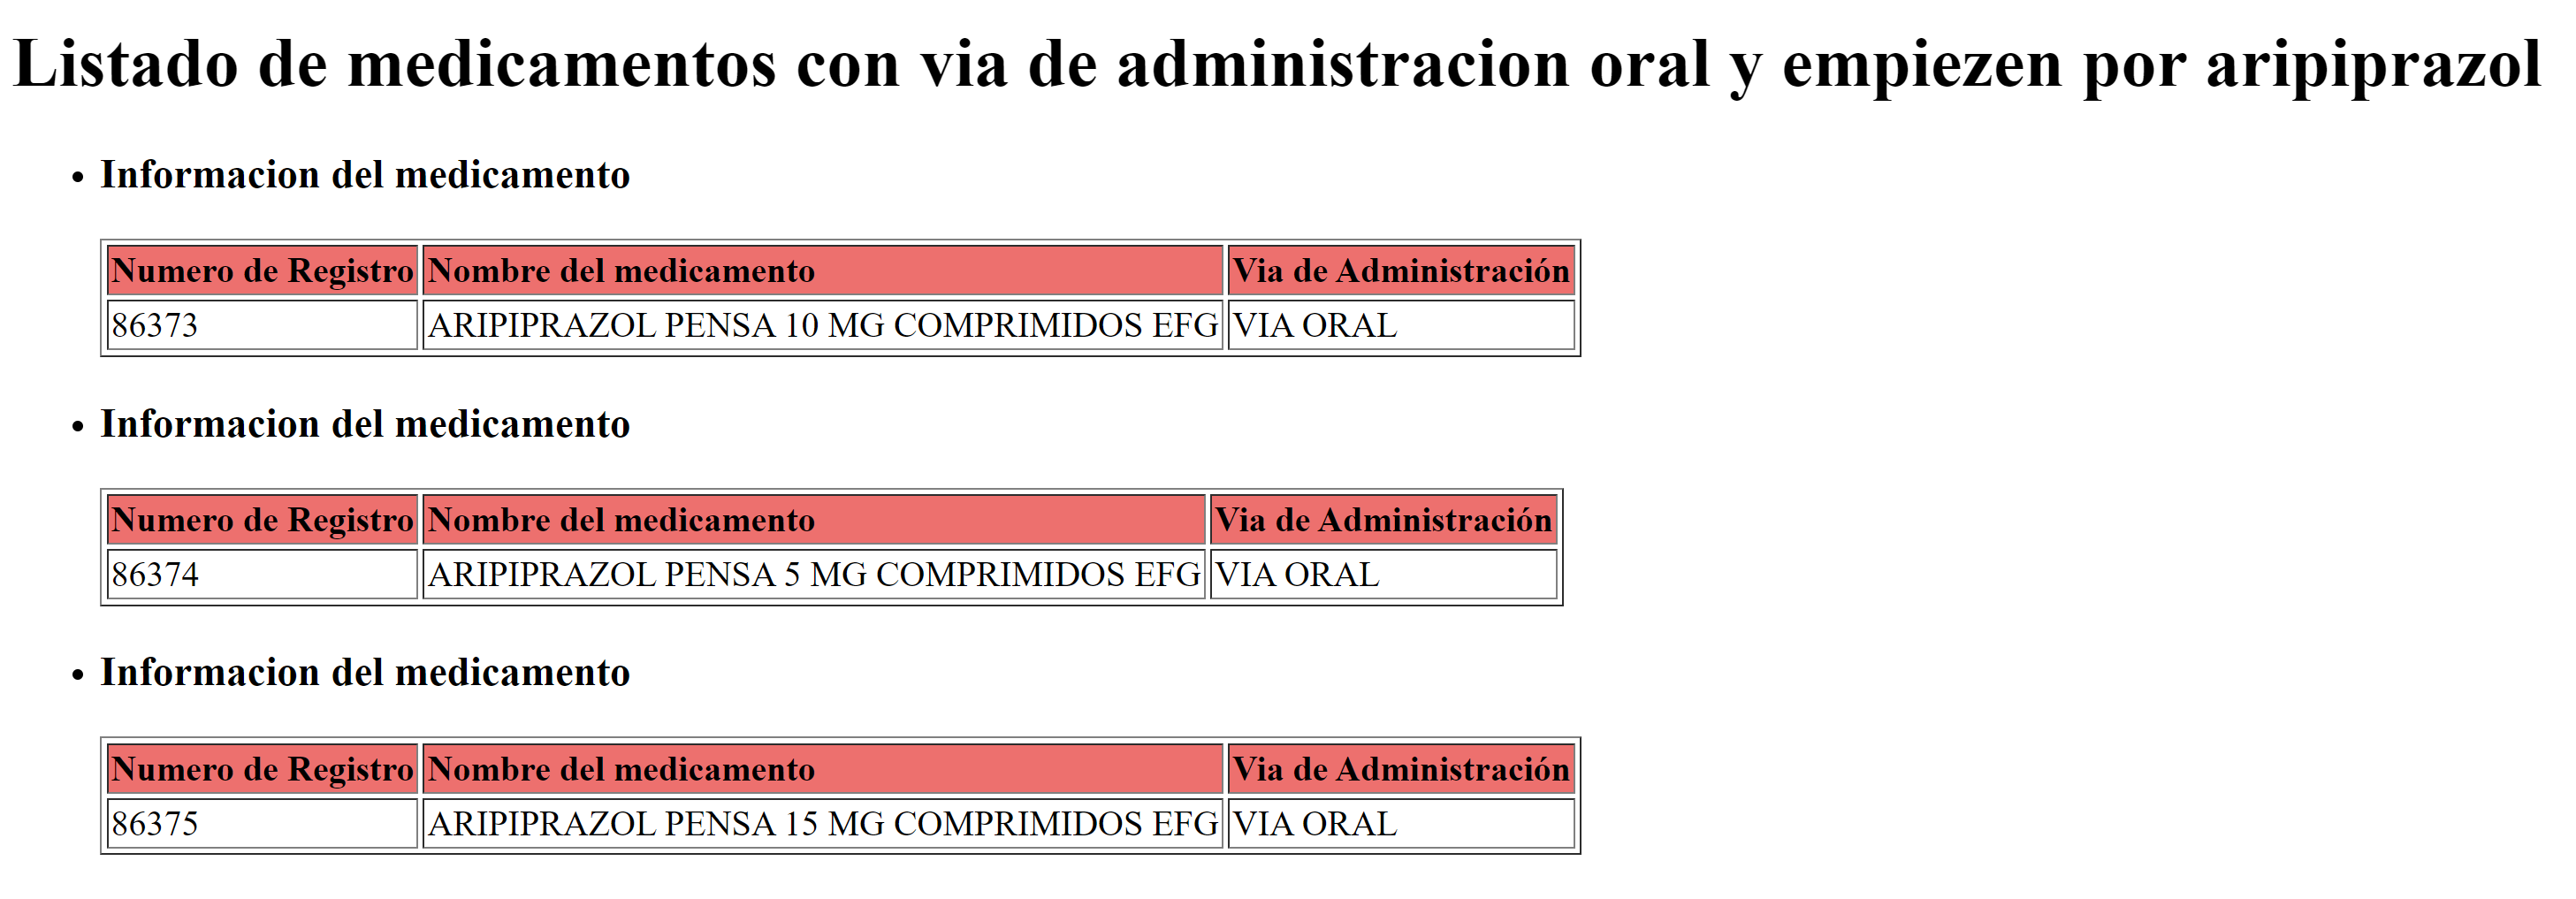
\includegraphics[scale=0.3]{images/html_output2.png}
    \caption{Archivo html resultante al aplicar la segunda transformación}
    \label{fig:mesh1}
\end{figure}


\subsection{Transformación 3}
La tercera transformación ayuda a obtener el listado de todos los medicamentos ordenados alfabéticamente que estén recubiertos por una película y sean de 500 mg

La transformación XSL que se ha realizado es la siguiente:
\begin{lstlisting}
<?xml version="1.0" encoding="UTF-8"?>

<xsl:stylesheet xmlns:xsl="http://www.w3.org/1999/XSL/Transform" version="1.0">
    <xsl:template match="/">
        <html>
            <body>
                <h1> Listado de medicamentos recubiertos con pelicula de dosis de 500 mg ordenados alfabeticamente</h1>
                <ul>
                    <xsl:for-each select="dataset/record">
                    <xsl:sort order="ascending" select="MEDICAMENTO"/>
                        <xsl:if test="contains(FORMA_FARMACEUTICA,'COMPRIMIDO RECUBIERTO CON PELICULA') ">
                            <xsl:if test="contains(DOSIS,'500 mg') ">
                                <li>
                                    <h3> Informacion del medicamento </h3>
                                    <table border="1">
                                        <tr bgcolor="#ff6d6d">
                                            <th> Numero de Registro</th>
                                            <th> Nombre del medicamento</th>
                                        </tr>
                                        <tr>
                                            <td>
                                                <xsl:value-of select="NUMERO_DE_REGISTRO"/>
                                            </td>
                                            <td>
                                                 <xsl:value-of select="MEDICAMENTO"/>
                                            </td>
                                        </tr>

                                    </table>
                                </li>
                            </xsl:if>
                        </xsl:if>
                    </xsl:for-each>
                </ul>
            </body>
        </html>
    </xsl:template>
</xsl:stylesheet>
\end{lstlisting}
Una vez aplicada la transformación al documento XML dónde se encuentran toda la información de los medicamentos, se muestra el siguiente html:

\begin{figure}[h]
    \centering
    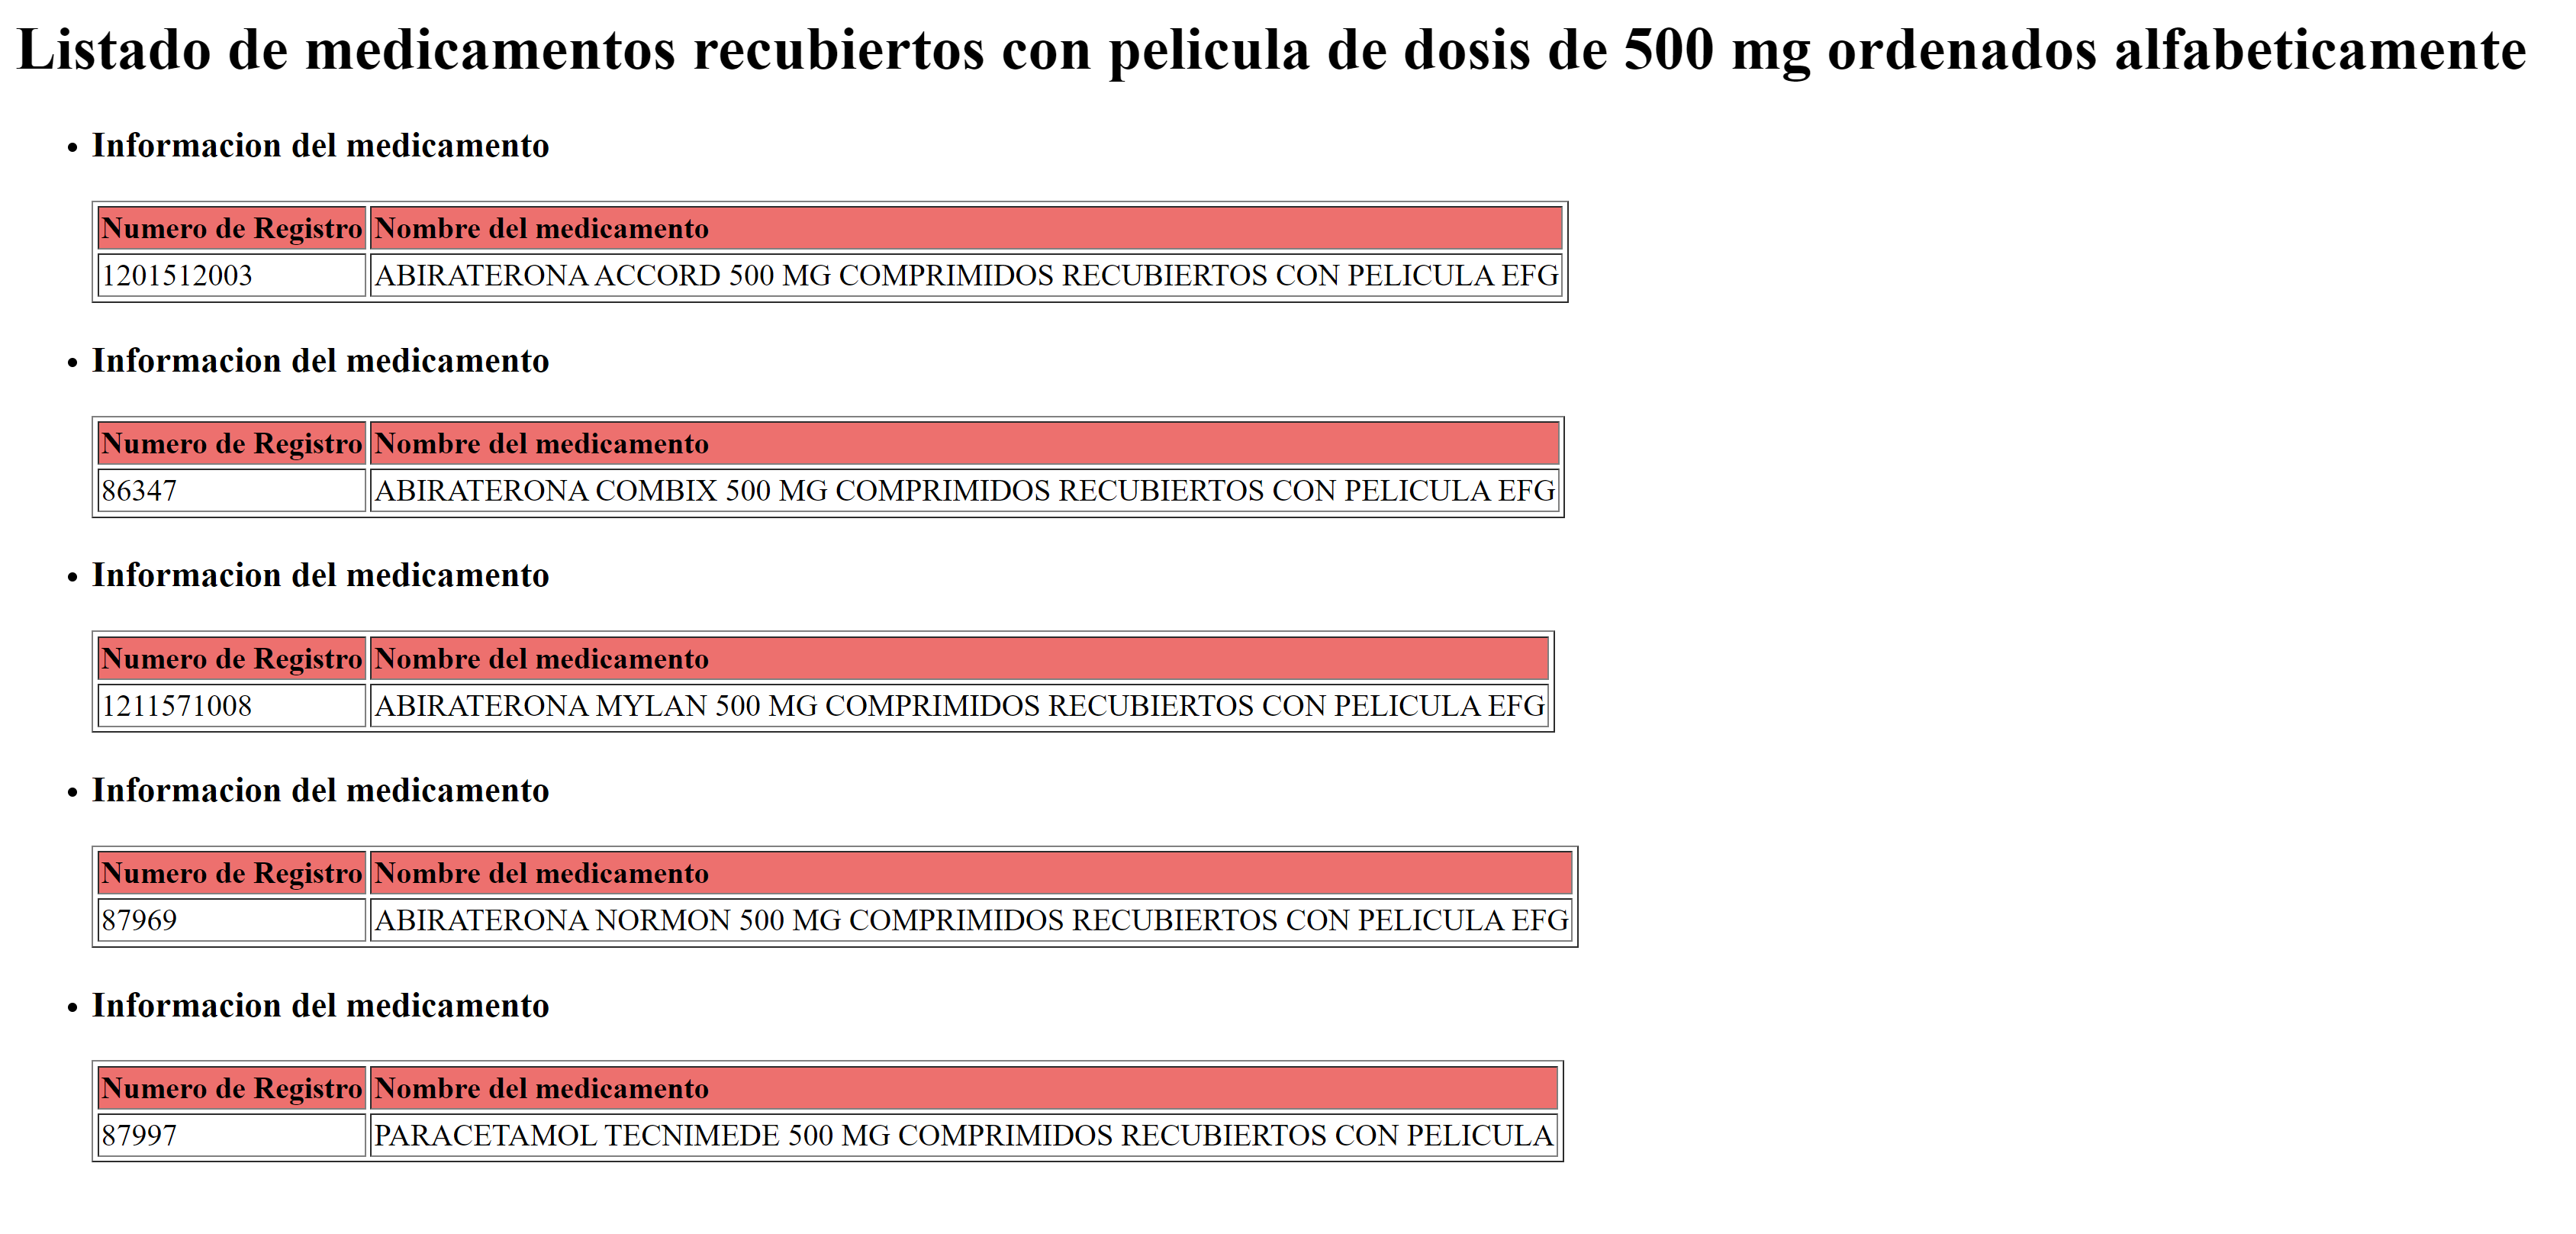
\includegraphics[scale=0.2]{images/html_output3.png}
    \caption{Archivo html resultante al aplicar la tercera transformación}
    \label{fig:mesh1}
\end{figure}






\end{document}